\documentclass[11pt,twocolumn]{article}

% ============================================================
% Packages
% ============================================================
\usepackage[utf8]{inputenc}
\usepackage[T1]{fontenc}
\usepackage{lmodern}
\usepackage[margin=1in]{geometry}
\usepackage{amsmath,amssymb,amsthm}
\usepackage{algorithm}
\usepackage{algpseudocode}
\usepackage{graphicx}
\usepackage{booktabs}
\usepackage{multirow}
\usepackage{array}
\usepackage{hyperref}
\usepackage{xcolor}
\usepackage{listings}
\usepackage{enumitem}
\usepackage{caption}
\usepackage{subcaption}
\usepackage{tikz}
\usepackage{float}
\usetikzlibrary{arrows.meta,positioning,shapes.geometric,fit,calc,decorations.pathreplacing}

% ============================================================
% Hyperref config
% ============================================================
\hypersetup{
  colorlinks=true,
  linkcolor=blue!70!black,
  citecolor=blue!70!black,
  urlcolor=blue!70!black,
}

% ============================================================
% Listings config
% ============================================================
\lstset{
  basicstyle=\ttfamily\scriptsize,
  breaklines=true,
  frame=single,
  numbers=left,
  numberstyle=\tiny\color{gray},
  keywordstyle=\color{blue!70!black}\bfseries,
  commentstyle=\color{green!50!black}\itshape,
  stringstyle=\color{red!60!black},
  showstringspaces=false,
  tabsize=2,
}

% ============================================================
% Theorem environments
% ============================================================
\newtheorem{theorem}{Theorem}[section]
\newtheorem{lemma}[theorem]{Lemma}
\newtheorem{corollary}[theorem]{Corollary}
\newtheorem{proposition}[theorem]{Proposition}
\newtheorem{definition}[theorem]{Definition}
\newtheorem{property}[theorem]{Property}
\newtheorem{invariant}[theorem]{Invariant}
\newtheorem{remark}[theorem]{Remark}

\theoremstyle{definition}
\newtheorem{example}[theorem]{Example}

% ============================================================
% Custom commands
% ============================================================
\newcommand{\bps}{\text{bps}}
\newcommand{\Gov}{\mathcal{G}}
\newcommand{\Signer}{\mathcal{S}}
\newcommand{\Chain}{\mathcal{C}}
\newcommand{\Fee}{\mathcal{F}}
\newcommand{\Strategy}{\mathcal{Y}}
\newcommand{\SAB}{\text{SAB}}
\newcommand{\halal}{\textsc{Halal}}
\newcommand{\haram}{\textsc{Haram}}
\newcommand{\cond}{\textsc{Conditional}}
\newcommand{\xLUX}{\texttt{xLUX}}

% ============================================================
% Title
% ============================================================
\title{
  \textbf{Sovereign DeFi: Per-Chain Governance, Shariah Compliance,\\
  and Securities-Compatible Cross-Chain Infrastructure} \\[6pt]
  \large Formal Governance Isolation, Islamic Finance Classification,\\
  and ERC-3643 Compliance in Lux Teleport
}

\author{
  Zach Kelling\thanks{Corresponding author: \texttt{zach@lux.network}} \quad
  Vishnu Seesahai \\
  \textit{Lux Industries} \\
  \texttt{research@lux.network} \\[4pt]
  \small Version 1.0 --- April 2025
}

\date{2022 (Revised December 2025)}

\begin{document}
\luxcoverpage
\maketitle

% ============================================================
% Abstract
% ============================================================
\begin{abstract}
Cross-chain bridge protocols concentrate governance power in a single entity that controls economic parameters across all connected chains. This paper presents Sovereign DeFi, a governance and compliance architecture for the Lux Teleport protocol that achieves three properties simultaneously: (1)~\emph{governance sovereignty}, where each chain's native token holders independently control their bridge instance's fees, limits, and yield strategy routing; (2)~\emph{protocol-level Shariah compliance}, where an on-chain classification contract enforces Islamic finance law by filtering yield sources into Halal, Haram, and Conditional categories under the authority of a Shariah Advisory Board multisig; and (3)~\emph{securities compatibility}, where ERC-3643 compliance registries ensure that regulated security tokens maintain jurisdictional, lockup, and accreditation constraints when teleported across chains. We prove a governance isolation theorem showing that a compromised governor on one chain cannot affect any other chain's bridge instance. We formalize the Shariah classification algebra, the securities compliance state machine, and the fee competition game between sovereign instances. We derive a Nash equilibrium for optimal fee setting and analyze the xLUX flywheel dynamics that emerge from fee aggregation across sovereign instances. The architecture enables any L1 or L2 to deploy a sovereign bridge instance that captures its own fee revenue while sharing the security of a unified MPC threshold signature network.
\end{abstract}

% ============================================================
\section{Introduction}
\label{sec:intro}
% ============================================================

Bridge governance is an unsolved problem. Existing cross-chain protocols fall into two categories: (a)~centrally governed bridges where a single team controls fees, token listings, and yield strategies across all chains (Wormhole~\cite{wormhole}, LayerZero~\cite{layerzero}), and (b)~ungoverned bridges where parameters are immutable at deployment, preventing adaptation to market conditions or regulatory requirements (tBTC~\cite{tbtc}).

Neither model serves the emerging requirements of cross-chain DeFi:

\begin{enumerate}[nosep]
  \item \textbf{Sovereignty}: Chain communities demand control over their own economic parameters. A Lux C-Chain bridge should be governed by LUX holders, not by a separate governance token.
  \item \textbf{Islamic finance}: Approximately 1.8~billion Muslims are excluded from DeFi because yield sources derive from interest (\emph{riba}), which Shariah law prohibits~\cite{usmani2002}. No existing bridge protocol provides protocol-level Shariah enforcement.
  \item \textbf{Securities regulation}: The EU Markets in Crypto-Assets regulation (MiCA)~\cite{mica2023} and US securities law require that security tokens maintain compliance constraints (accreditation, lockup, jurisdiction) across chain boundaries. Existing bridges strip these constraints during transfer.
\end{enumerate}

Lux Teleport's Sovereign DeFi architecture addresses all three requirements through a clean separation of three authority domains---security, economics, and protocol---where each domain has well-defined capabilities and hard limits that cannot be overridden by any other domain.

\paragraph{Contributions.} This paper makes six contributions:
\begin{enumerate}[nosep]
  \item A formal governance model with proven isolation properties (Section~\ref{sec:governance}).
  \item A Shariah compliance algebra with on-chain enforcement (Section~\ref{sec:shariah}).
  \item A securities compliance state machine compatible with ERC-3643~\cite{erc3643} (Section~\ref{sec:securities}).
  \item A white-label architecture enabling sovereign deployment (Section~\ref{sec:whitelabel}).
  \item Formal proofs of governance isolation, exit guarantee, and fee cap invariants (Section~\ref{sec:formal}).
  \item A game-theoretic analysis of fee competition between sovereign instances (Section~\ref{sec:economics}).
\end{enumerate}

% ============================================================
\section{System Model}
\label{sec:system}
% ============================================================

\subsection{Entities}

\begin{definition}[MPC Signer Set]
\label{def:signer}
A set $\Signer = \{s_1, \ldots, s_n\}$ of $n$ threshold signature nodes. A threshold $t \leq n$ defines the minimum quorum for valid signatures. The default configuration is $n = 3, t = 2$. The signer set authorizes mint and release operations via FROST~\cite{frost} (Ed25519/Schnorr chains) or CGGMP21~\cite{cggmp21} (secp256k1 chains).
\end{definition}

\begin{definition}[Sovereign Governor]
\label{def:governor}
For chain $\Chain_i$, the governor $\Gov_i$ is the on-chain address (DAO timelock, multisig, or single owner) that controls economic parameters of the bridge instance on $\Chain_i$. The governor is set by the chain's native token holders through their existing governance mechanism.
\end{definition}

\begin{definition}[OmnichainRouter Instance]
\label{def:router}
An immutable smart contract $R_i$ deployed on chain $\Chain_i$ that: (a)~verifies MPC threshold signatures, (b)~tracks per-source-chain nonce bitmaps, (c)~enforces fee caps and daily limits, and (d)~routes yield strategy deposits. Each instance is independently parameterized by its governor $\Gov_i$.
\end{definition}

\begin{definition}[Shariah Advisory Board]
\label{def:sab}
A $k$-of-$m$ multisig $\SAB$ of recognized Islamic finance scholars who classify yield strategies. The SAB operates independently of both the MPC signer set and chain governors.
\end{definition}

\subsection{Authority Domains}

Teleport cleanly separates three authority domains with non-overlapping capabilities:

\begin{table}[h]
\centering
\small
\begin{tabular}{@{}p{1.5cm}p{2.5cm}p{2.8cm}@{}}
\toprule
\textbf{Domain} & \textbf{Controller} & \textbf{Scope} \\
\midrule
Security & MPC signer set $\Signer$ & Mint/release authorization, signer rotation \\
\addlinespace
Economics & Chain governor $\Gov_i$ & Fees, limits, strategies, Shariah mode \\
\addlinespace
Protocol & Immutable code & Nonce checks, signature verification, fee cap \\
\addlinespace
Compliance & SAB multisig & Yield strategy Shariah classification \\
\bottomrule
\end{tabular}
\caption{Authority domain separation. No domain can override another.}
\label{tab:separation}
\end{table}

\subsection{Threat Model}

We assume a computationally bounded adversary $\mathcal{A}$ who may:
\begin{itemize}[nosep]
  \item Compromise up to $t - 1$ MPC signer nodes
  \item Capture the governor address on any single chain $\Chain_i$
  \item Corrupt up to $k - 1$ SAB members
  \item Observe and reorder transactions on any chain
  \item Deploy malicious bridge instances mimicking Teleport
\end{itemize}

The adversary \emph{cannot}:
\begin{itemize}[nosep]
  \item Compromise $\geq t$ MPC signer nodes simultaneously
  \item Break ECDSA, Ed25519, or Schnorr hardness assumptions
  \item Rewrite confirmed blocks on connected chains
  \item Modify deployed immutable contract bytecode
\end{itemize}

% ============================================================
\section{Sovereign Governance}
\label{sec:governance}
% ============================================================

\subsection{Governance Instantiation}

Each chain $\Chain_i$ that connects to Teleport deploys an OmnichainRouter instance $R_i$ with a designated governor $\Gov_i$. The governor is typically:

\begin{itemize}[nosep]
  \item \textbf{Lux C-Chain}: LUX token DAO with 48-hour timelock. Fees flow to xLUX holders.
  \item \textbf{Zoo EVM}: ZOO token governance. Fees flow to ZOO stakers.
  \item \textbf{External L1/L2}: The chain's own governance mechanism, chosen at deployment.
\end{itemize}

\noindent
The key insight is that $\Gov_i$ controls \emph{only} the economic parameters of $R_i$. It has no authority over $R_j$ for $j \neq i$, and no authority over the MPC signer set or immutable protocol logic.

\subsection{Governor Capability Matrix}

\begin{table}[h]
\centering
\small
\begin{tabular}{@{}p{3.8cm}cc@{}}
\toprule
\textbf{Action} & \textbf{CAN} & \textbf{CANNOT} \\
\midrule
Set bridge fee (0--100 bps) & $\checkmark$ & \\
Set daily mint limits & $\checkmark$ & \\
Register new bridge tokens & $\checkmark$ & \\
Enable Shariah mode & $\checkmark$ & \\
Set yield strategy routing & $\checkmark$ & \\
Change fee recipient (48h lock) & $\checkmark$ & \\
Transfer governance (2-step) & $\checkmark$ & \\
\midrule
Mint bridge tokens & & $\times$ \\
Modify nonce bitmaps & & $\times$ \\
Set fee $> 100$ bps & & $\times$ \\
Bypass signature verification & & $\times$ \\
Upgrade contract bytecode & & $\times$ \\
Override signer rotation & & $\times$ \\
Access other chains' $R_j$ & & $\times$ \\
\bottomrule
\end{tabular}
\caption{Governor capability matrix. The ``CANNOT'' column represents hard-coded invariants enforced at the bytecode level, not merely policy.}
\label{tab:capability}
\end{table}

\subsection{Fee Configuration}

The governor sets the bridge fee rate $f_b$ and stakeholder share $f_s$:

\begin{equation}
  0 \leq f_b \leq 100 \text{ bps}, \quad 0 \leq f_s \leq 10{,}000 \text{ bps}
\end{equation}

The hard cap $f_b \leq 100$ bps (1\%) is enforced at the bytecode level:

\begin{lstlisting}[language=Solidity,caption=Fee cap enforcement]
function setBridgeFee(uint256 newFeeBps)
    external onlyGovernor
{
    require(
        newFeeBps <= MAX_FEE_BPS,
        "fee exceeds hard cap"
    );
    // MAX_FEE_BPS = 100, immutable
    bridgeFeeBps = newFeeBps;
    emit BridgeFeeUpdated(newFeeBps);
}
\end{lstlisting}

\noindent
The constant \texttt{MAX\_FEE\_BPS = 100} is defined at compile time and cannot be modified post-deployment, even by the governor.

\subsection{Fee Distribution}

For a bridge operation of amount $a$ on chain $\Chain_i$ with fee rate $f_b^{(i)}$ and stakeholder share $f_s^{(i)}$:

\begin{align}
  \text{fee} &= a \cdot \frac{f_b^{(i)}}{10{,}000} \\
  \text{toStakeholders} &= \text{fee} \cdot \frac{f_s^{(i)}}{10{,}000} \\
  \text{toTreasury} &= \text{fee} - \text{toStakeholders}
\end{align}

Each chain instance independently determines where fees flow:
\begin{itemize}[nosep]
  \item On Lux C-Chain: stakeholder vault $=$ xLUX (LiquidLUX).
  \item On Zoo EVM: stakeholder vault $=$ ZOO staking contract.
  \item On white-label deployments: stakeholder vault $=$ deployer-designated address.
\end{itemize}

\subsection{Signer Rotation Protection}

MPC signer rotation is the highest-severity operation. The rotation delay is a configurable operational parameter (default 24h, governor-settable $\in [0, 7\text{d}]$), not a security invariant---the MPC threshold \emph{is} the trust model. A compromised governor cannot initiate rotation; only the current $t$-of-$n$ MPC set can.

\begin{enumerate}[nosep]
  \item Current $t$-of-$n$ MPC set signs the rotation proposal with the new MPC group address.
  \item Configurable delay begins (default 24h). Pending signers are published on-chain.
  \item During the delay, users may exit by burning bridge tokens for underlying assets.
  \item After the delay expires, any address may execute the rotation.
  \item Current signers may cancel during the delay period.
\end{enumerate}

\begin{property}[Exit Window]
\label{prop:exit}
For any signer rotation event at time $t_0$ with rotation delay $\delta$ (default 24h, max 7 days), every bridge token holder has the interval $[t_0, t_0 + \delta)$ to exit the system by burning bridge tokens and receiving the underlying asset at the current share price.
\end{property}

% ============================================================
\section{Shariah Compliance}
\label{sec:shariah}
% ============================================================

\subsection{Islamic Finance Fundamentals}

Islamic finance law (Shariah) governs financial transactions for approximately 1.8~billion Muslims worldwide~\cite{usmani2002}. The core prohibitions relevant to DeFi are:

\begin{definition}[Shariah Prohibitions in Finance]
\label{def:prohibitions}
\begin{enumerate}[nosep]
  \item \textbf{Riba} (interest/usury): Any guaranteed return on capital without bearing risk. Lending at interest is categorically prohibited~\cite{iqbal2011}.
  \item \textbf{Gharar} (excessive uncertainty): Contracts with material ambiguity in terms, subject matter, or execution~\cite{elgari2003}.
  \item \textbf{Maysir} (gambling): Zero-sum speculative transactions with no underlying economic activity.
\end{enumerate}
\end{definition}

Critically, Shariah does \emph{not} prohibit profit. Fee-based revenue, profit-sharing arrangements (\emph{mudarabah}), and trade-based financing (\emph{murabahah}) are permitted~\cite{usmani2002}. The distinction is between earning returns from productive activity (permitted) and earning returns from money itself (prohibited).

\subsection{Classification Algebra}

We define a formal classification system for yield sources:

\begin{definition}[Compliance Status]
\label{def:compliance}
The Shariah classification function $\phi: \Strategy \to \{\halal, \haram, \cond, \textsc{Review}\}$ maps each yield strategy to a compliance status:
\begin{itemize}[nosep]
  \item $\halal$: Fee-based or profit-sharing yield. No interest component.
  \item $\haram$: Interest-based yield. Contains riba.
  \item $\cond$: Contains mixed sources. Permissible if the interest component is purified (donated to charity).
  \item $\textsc{Review}$: Pending SAB classification. Treated as $\haram$ by default.
\end{itemize}
\end{definition}

\begin{definition}[Shariah Filter]
\label{def:filter}
The ShariaFilter contract enforces the classification:
\begin{equation}
  \text{deposit}(y, a) =
  \begin{cases}
    \text{execute} & \text{if } \neg\texttt{shariahMode} \\
    \text{execute} & \text{if } \phi(y) = \halal \\
    \text{revert} & \text{otherwise}
  \end{cases}
\end{equation}
where $y \in \Strategy$ is the strategy and $a$ is the deposit amount.
\end{definition}

The filter is applied at the vault level: when Shariah mode is enabled on a bridge instance, only Halal-classified strategies receive deposits. The filter does not affect bridge operations (lock/mint/burn/release), only yield routing.

\subsection{Classification Table}

Table~\ref{tab:shariah-full} presents the complete classification of yield sources available to Teleport bridge vaults.

\begin{table*}[t]
\centering
\small
\begin{tabular}{@{}llllp{5.5cm}@{}}
\toprule
\textbf{Strategy} & \textbf{Protocol} & \textbf{APY} & \textbf{Status} & \textbf{Shariah Rationale} \\
\midrule
\multicolumn{5}{@{}l}{\textbf{Halal --- Fee-Based and Profit-Sharing Yield}} \\
\addlinespace
DEX trading fees & Uniswap, Curve & 5--20\% & \halal & Service fee for liquidity provision; no lending \\
Bridge fees & Teleport & 0.5--2\% & \halal & Service fee for cross-chain transfer \\
Validator staking & Lux, Ethereum & 3--5\% & \halal & Profit-sharing for network security service \\
LP provision & Pendle, Convex & 5--15\% & \halal & Profit-sharing from trading activity \\
Perpetuals fees & LPX Perps & 10--30\% & \halal & Fee revenue from derivatives market-making \\
BTC staking & Babylon, Lombard & 3--12\% & \halal & Security provision, not lending \\
Solana staking & Marinade, Jito & 5--10\% & \halal & Validator delegation rewards \\
TON staking & Tonstakers, Bemo & 5--15\% & \halal & Network validation, fee-based \\
Restaking & EigenLayer, Symbiotic & 3--8\% & \halal & Security provision for AVS operators \\
\midrule
\multicolumn{5}{@{}l}{\textbf{Haram --- Interest-Based Yield}} \\
\addlinespace
Lending interest & Aave, Morpho & 2--12\% & \haram & Direct riba: guaranteed interest on loaned capital \\
Lending interest & Compound & 2--8\% & \haram & Direct riba: interest accrual on supplied assets \\
Savings rate & MakerDAO/Sky DSR & 5--8\% & \haram & Interest-bearing deposit mechanism \\
Leveraged farming & Various & 10--40\% & \haram & Riba-amplified through leverage \\
Interest stables & sDAI, aUSDC & 4--8\% & \haram & Yield derived from underlying lending \\
\midrule
\multicolumn{5}{@{}l}{\textbf{Conditional --- Requires Purification}} \\
\addlinespace
Mixed LP & Curve 3pool & 3--10\% & \cond & Contains fee component (halal) and lending component (haram); permissible if interest portion donated \\
RWA yield & Ondo, Centrifuge & 4--8\% & \cond & Depends on underlying asset structure \\
\bottomrule
\end{tabular}
\caption{Complete Shariah classification of yield strategies available to Teleport bridge vaults. Classifications are determined by the Shariah Advisory Board and enforced on-chain by the ShariaFilter contract.}
\label{tab:shariah-full}
\end{table*}

\subsection{Shariah Advisory Board Governance}

The SAB operates as a $k$-of-$m$ multisig (default $k=3, m=5$) with the following constraints:

\begin{enumerate}[nosep]
  \item SAB members must hold recognized Islamic finance certification (CSAA, CIFE, or equivalent)~\cite{aaoifi2015}.
  \item Classification updates require $k$ signatures and a 48-hour timelock.
  \item The SAB can only modify $\phi(y)$ for specific strategies; it cannot modify the filter logic itself.
  \item Only the SAB can change SAB membership---the governor and admin roles have no authority over SAB composition. This prevents governance capture of Shariah compliance.
  \item SAB member rotation follows a 2-step process with a 30-day notice period.
  \item All classification decisions are recorded on-chain with rationale hashes referencing IPFS-hosted fatwa documents.
\end{enumerate}

\begin{lstlisting}[language=Solidity,caption=ShariaFilter classification update]
function updateClassification(
    address strategy,
    ComplianceStatus newStatus,
    bytes32 fatwaHash
) external onlySAB timelocked(48 hours) {
    require(
        newStatus != ComplianceStatus.Review,
        "cannot set Review"
    );
    classifications[strategy] = Classification({
        status: newStatus,
        fatwaHash: fatwaHash,
        updatedAt: block.timestamp,
        sabSignatures: msg.data
    });
    emit ClassificationUpdated(
        strategy, newStatus, fatwaHash
    );
}
\end{lstlisting}

\subsection{Purification Mechanism}

For Conditional strategies, the protocol implements automatic purification:

\begin{equation}
  \text{purified} = \text{yield} - \text{yield} \cdot r_{\text{interest}}
\end{equation}

where $r_{\text{interest}}$ is the estimated interest ratio (set by the SAB). The interest portion is automatically directed to a charity address designated by the SAB. This follows the AAOIFI standard on income purification~\cite{aaoifi2015}.

\subsection{Impact Assessment}

The Islamic finance market represents \$3.96~trillion in assets globally~\cite{ifdi2024}. Approximately 800~million Muslims lack access to formal financial services~\cite{worldbank2022}. Protocol-level Shariah compliance eliminates the need for individual users to evaluate each yield source against Islamic law, removing a significant barrier to DeFi adoption:

\begin{itemize}[nosep]
  \item Users enable Shariah mode once; the protocol enforces compliance thereafter.
  \item SAB-certified classifications provide scholarly authority comparable to traditional Islamic banking.
  \item On-chain fatwa references create an auditable compliance trail.
  \item No trust in the bridge operator is required---the filter is enforced at the smart contract level.
\end{itemize}

% ============================================================
\section{Securities Compliance}
\label{sec:securities}
% ============================================================

\subsection{The Cross-Chain Securities Problem}

Security tokens issued under ERC-3643 (T-REX)~\cite{erc3643} maintain on-chain compliance registries that enforce:

\begin{enumerate}[nosep]
  \item \textbf{Investor identity}: KYC/AML verified addresses in an identity registry.
  \item \textbf{Jurisdiction}: Country-level transfer restrictions (e.g., US accredited investors only).
  \item \textbf{Lockup}: Time-based transfer restrictions (e.g., 12-month hold after issuance).
  \item \textbf{Accreditation}: Investor qualification (e.g., net worth, income thresholds).
  \item \textbf{Capacity}: Maximum number of holders or per-holder limits.
\end{enumerate}

When a security token is bridged via a conventional protocol, these constraints are stripped. The bridge token on the destination chain has no compliance registry, enabling unrestricted transfer to non-qualified addresses. This violates securities law in every major jurisdiction.

\subsection{Compliance-Preserving Teleport}

Teleport introduces a compliance-preserving bridge mode for ERC-3643 tokens:

\begin{definition}[Securities Bridge Mode]
\label{def:securities}
For a security token $T$ with compliance registry $\mathcal{R}_T$ on source chain $\Chain_s$, the securities bridge mode:
\begin{enumerate}[nosep]
  \item Deploys a mirrored compliance registry $\mathcal{R}_T'$ on destination chain $\Chain_d$.
  \item The MPC signer set attests to registry state, synchronizing $\mathcal{R}_T'$ with $\mathcal{R}_T$.
  \item The bridge token on $\Chain_d$ enforces the same transfer restrictions as $T$ on $\Chain_s$.
  \item Registry updates propagate cross-chain within one attestation period.
\end{enumerate}
\end{definition}

\subsection{Compliance State Machine}

Each security token transfer follows a state machine with compliance checks at every transition:

\begin{figure}[h]
\centering
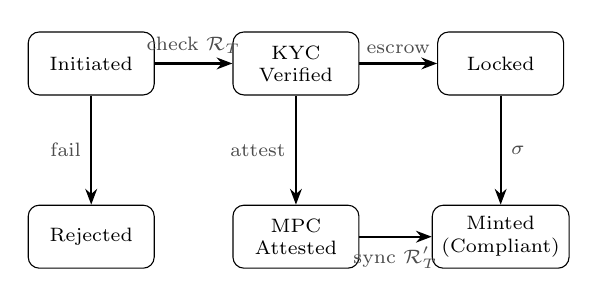
\begin{tikzpicture}[
  node distance=1.8cm,
  state/.style={rectangle, rounded corners, draw, minimum width=1.6cm, minimum height=0.8cm, font=\scriptsize, align=center},
  arrow/.style={-{Stealth[length=2mm]}, thick},
  label/.style={font=\scriptsize, text=black!70}
]
  \node[state] (init) {Initiated};
  \node[state, right of=init, xshift=0.8cm] (kyc) {KYC\\Verified};
  \node[state, right of=kyc, xshift=0.8cm] (lock) {Locked};
  \node[state, below of=kyc, yshift=-0.4cm] (attest) {MPC\\Attested};
  \node[state, below of=lock, yshift=-0.4cm] (mint) {Minted\\(Compliant)};
  \node[state, below of=init, yshift=-0.4cm] (reject) {Rejected};

  \draw[arrow] (init) -- node[above, label] {check $\mathcal{R}_T$} (kyc);
  \draw[arrow] (kyc) -- node[above, label] {escrow} (lock);
  \draw[arrow] (lock) -- node[right, label] {$\sigma$} (mint);
  \draw[arrow] (kyc) -- node[left, label] {attest} (attest);
  \draw[arrow] (attest) -- node[below, label] {sync $\mathcal{R}_T'$} (mint);
  \draw[arrow] (init) -- node[left, label] {fail} (reject);
\end{tikzpicture}
\caption{Securities compliance state machine. Transfers require KYC verification on both source and destination chains before minting.}
\label{fig:compliance-sm}
\end{figure}

\subsection{Compliance Registry Interface}

\begin{lstlisting}[language=Solidity,caption=IComplianceRegistry interface]
interface IComplianceRegistry {
    // Identity verification
    function isVerified(address investor)
        external view returns (bool);
    function getCountry(address investor)
        external view returns (uint16);

    // Transfer compliance
    function canTransfer(
        address from,
        address to,
        uint256 amount
    ) external view returns (bool);

    // Lockup enforcement
    function getLockupEnd(address investor)
        external view returns (uint256);

    // Accreditation
    function isAccredited(address investor)
        external view returns (bool);

    // Capacity
    function holderCount()
        external view returns (uint256);
    function maxHolders()
        external view returns (uint256);
}
\end{lstlisting}

\subsection{Settlement Registry}

For regulatory reporting, Teleport maintains a settlement registry that records every cross-chain security token transfer with sufficient detail for audit:

\begin{definition}[Settlement Record]
\label{def:settlement}
A settlement record $\rho = (T, \Chain_s, \Chain_d, \text{from}, \text{to}, a, t, \sigma, \text{complianceHash})$ contains the token, source and destination chains, sender, recipient, amount, timestamp, MPC signature, and a hash of the compliance state at the time of transfer.
\end{definition}

The settlement registry is append-only and indexed by token address and time range. Regulators can query the registry to reconstruct the complete transfer history of any security token across all chains.

\subsection{Regulatory Compatibility}

\begin{table}[h]
\centering
\small
\begin{tabular}{@{}p{2cm}p{4.8cm}@{}}
\toprule
\textbf{Regulation} & \textbf{Teleport Compliance Mechanism} \\
\midrule
MiCA~\cite{mica2023} & Cross-chain identity registry sync, transaction reporting via settlement registry \\
\addlinespace
SEC Reg D & Accredited investor checks enforced on destination chain; lockup periods preserved \\
\addlinespace
SEC Reg S & Country-code transfer restrictions; US persons blocked on non-exempt chains \\
\addlinespace
AAOIFI & ShariaFilter + SAB classifications; on-chain fatwa references \\
\addlinespace
ERC-3643 & Full T-REX registry mirroring; compliance agent role preserved cross-chain \\
\bottomrule
\end{tabular}
\caption{Regulatory framework compatibility.}
\label{tab:regulatory}
\end{table}

% ============================================================
\section{White-Label Architecture}
\label{sec:whitelabel}
% ============================================================

\subsection{Shared Security, Sovereign Economics}

The white-label architecture enables any L1, L2, or application chain to deploy a sovereign bridge instance that:

\begin{enumerate}[nosep]
  \item Shares the security of the unified MPC signer set (no additional trust assumptions).
  \item Captures its own bridge fee revenue (not shared with other instances).
  \item Independently governs fees, limits, token listings, and compliance modes.
  \item Uses its own branding, domain, and user interface.
\end{enumerate}

\begin{figure}[h]
\centering
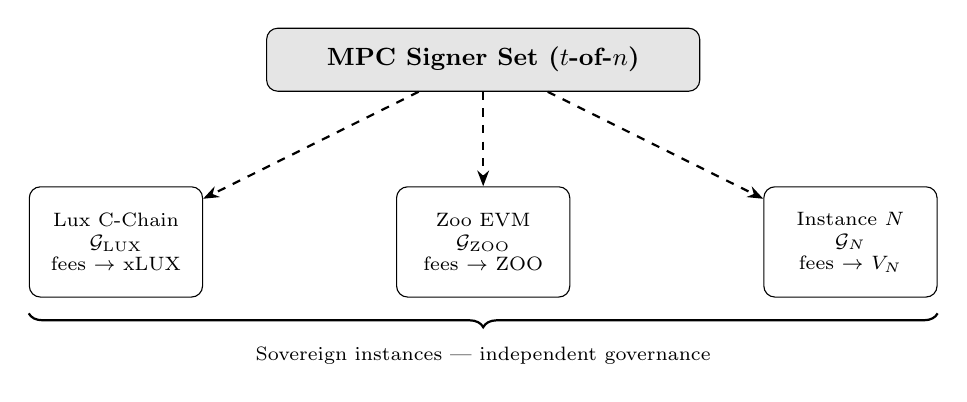
\begin{tikzpicture}[
  node distance=1.5cm,
  mpc/.style={rectangle, rounded corners, draw, fill=black!10, minimum width=5.5cm, minimum height=0.8cm, font=\small\bfseries},
  inst/.style={rectangle, rounded corners, draw, minimum width=2.2cm, minimum height=1.4cm, font=\scriptsize, align=center},
  arrow/.style={-{Stealth[length=2mm]}, thick, dashed},
]
  \node[mpc] (mpc) {MPC Signer Set ($t$-of-$n$)};

  \node[inst, below left=1.2cm and 0.8cm of mpc] (lux)
    {Lux C-Chain\\$\Gov_{\text{LUX}}$\\fees $\to$ xLUX};
  \node[inst, below=1.2cm of mpc] (zoo)
    {Zoo EVM\\$\Gov_{\text{ZOO}}$\\fees $\to$ ZOO};
  \node[inst, below right=1.2cm and 0.8cm of mpc] (wl)
    {Instance $N$\\$\Gov_N$\\fees $\to$ $V_N$};

  \draw[arrow] (mpc) -- (lux);
  \draw[arrow] (mpc) -- (zoo);
  \draw[arrow] (mpc) -- (wl);

  \draw[decorate, decoration={brace, amplitude=5pt, mirror}, thick]
    ([yshift=-0.2cm]lux.south west) -- ([yshift=-0.2cm]wl.south east)
    node[midway, below=0.3cm, font=\scriptsize] {Sovereign instances --- independent governance};
\end{tikzpicture}
\caption{White-label architecture. A single MPC signer set secures all instances. Each instance has independent governance and fee capture.}
\label{fig:whitelabel}
\end{figure}

\subsection{Deployment Process}

A new sovereign instance requires:

\begin{enumerate}[nosep]
  \item Deploy OmnichainRouter with the chain's governor address.
  \item Deploy bridge tokens (yTokens) for each supported asset.
  \item Register the instance with the MPC coordinator (permissionless).
  \item Configure fee rate, stakeholder vault, and optional compliance modes.
\end{enumerate}

The protocol layer is branding-agnostic: the same MPC attestation that works for Lux bridge tokens works for any sovereign instance's tokens. The MPC network does not distinguish between instances---it verifies lock events and produces signatures regardless of which instance emitted the event.

\subsection{Instance Isolation}

\begin{theorem}[Instance Isolation]
\label{thm:instance}
For sovereign instances $R_i$ and $R_j$ on chains $\Chain_i$ and $\Chain_j$ respectively:
\begin{enumerate}[nosep]
  \item $\Gov_i$ has no write access to any storage slot of $R_j$.
  \item Fee parameters $(f_b^{(i)}, f_s^{(i)})$ are stored locally in $R_i$ and read only by $R_i$.
  \item Nonce bitmaps in $R_i$ are indexed by source chain; processing a nonce in $R_i$ does not affect the bitmap in $R_j$.
\end{enumerate}
\end{theorem}

\begin{proof}
Each $R_i$ is an independent contract deployment on chain $\Chain_i$. By the EVM execution model, contract storage is isolated per address: $\texttt{SSTORE}$ and $\texttt{SLOAD}$ operate on the calling contract's storage trie. The \texttt{onlyGovernor} modifier restricts parameter writes to $\Gov_i$, which is an address on $\Chain_i$ with no ability to submit transactions to $\Chain_j$ (different chain, different address space). Nonce bitmaps are per-contract state, and processing $(C_s, \nu)$ in $R_i$ writes to $R_i$'s storage, which is inaccessible to $R_j$.
\end{proof}

% ============================================================
\section{Formal Properties}
\label{sec:formal}
% ============================================================

\subsection{Governance Isolation Theorem}

\begin{theorem}[Governance Isolation]
\label{thm:gov-isolation}
Let $\Gov_i$ be the governor of chain $\Chain_i$'s bridge instance $R_i$. Even if $\Gov_i$ is fully compromised (adversary controls the governor key), the adversary cannot:
\begin{enumerate}[nosep]
  \item Mint bridge tokens on any chain without a valid MPC signature.
  \item Modify the nonce bitmap on any chain.
  \item Set $f_b^{(i)} > 100$ bps.
  \item Affect parameters of $R_j$ for any $j \neq i$.
  \item Bypass the 48-hour timelock on stakeholder vault changes.
\end{enumerate}
\end{theorem}

\begin{proof}
We prove each property:

\emph{(1)} The \texttt{bridgeMint} function requires $\texttt{ecrecover}(\sigma) = \texttt{mpcAddress}$. The governor address is checked against \texttt{governor}, not \texttt{mpcAddress}. No code path grants the governor mint authority. The \texttt{onlyGovernor} modifier gates only parameter-setting functions, which are disjoint from the mint/release code paths.

\emph{(2)} Nonce bitmaps are modified only within \texttt{bridgeMint} and \texttt{bridgeRelease}, both of which require valid MPC signatures. No governor-accessible function writes to the nonce bitmap mapping.

\emph{(3)} The \texttt{setBridgeFee} function contains \texttt{require(newFeeBps <= MAX\_FEE\_BPS)}. \texttt{MAX\_FEE\_BPS} is a compile-time constant set to 100. The \texttt{PUSH} opcode embeds this value directly in bytecode; it cannot be modified by any transaction.

\emph{(4)} Follows from Theorem~\ref{thm:instance}: each $R_j$ is a separate contract on a separate chain with independent storage.

\emph{(5)} The \texttt{setStakeholderVault} function stores the new vault address but does not activate it. A separate \texttt{executeVaultChange} function requires $\texttt{block.timestamp} \geq \texttt{vaultChangeTimestamp} + 48 \text{ hours}$. No code path bypasses this check.
\end{proof}

\subsection{Exit Guarantee}

\begin{theorem}[Exit Guarantee]
\label{thm:exit}
Under the assumption that at least $t$ of $n$ MPC signer nodes remain honest and the destination chain is live, any bridge token holder can exit the system (burn bridge tokens and receive underlying assets) within 7 days under all conditions, including:
\begin{enumerate}[nosep]
  \item Governor compromise on any chain.
  \item Single MPC node failure ($< t$ failures).
  \item Pending signer rotation.
  \item Shariah mode changes.
  \item Fee parameter changes.
\end{enumerate}
\end{theorem}

\begin{proof}
The \texttt{burnForWithdrawal} function is callable by any bridge token holder without governor approval. It emits a \texttt{Burn} event. The MPC signer set observes this event and, given $\geq t$ honest nodes, produces a release signature within one attestation period (15 minutes). The \texttt{bridgeRelease} function on the source chain verifies the signature and releases assets. Governor compromise does not affect this path because \texttt{burnForWithdrawal} has no \texttt{onlyGovernor} modifier, and \texttt{bridgeRelease} requires only a valid MPC signature.

During signer rotation, the 7-day timelock ensures that the current signer set remains active throughout the exit window. Shariah mode and fee changes affect only future deposits, not the burn/release path. Fee changes affect only the fee on the next bridge operation; they do not affect previously minted bridge tokens.
\end{proof}

\subsection{Fee Cap Invariant}

\begin{invariant}[Fee Cap]
\label{inv:feecap}
For all chains $\Chain_i$ and all times $t$:
\begin{equation}
  f_b^{(i)}(t) \leq 100 \text{ bps}
\end{equation}
This holds even if the governor is compromised, the MPC set is rotated, or the contract is called via a delegate call from a malicious contract.
\end{invariant}

\begin{proof}
The fee rate is stored as a \texttt{uint256} in contract storage. The only function that modifies this value is \texttt{setBridgeFee}, which contains the hard-coded check \texttt{require(newFeeBps <= 100)}. The constant 100 is embedded in the contract bytecode as a \texttt{PUSH1 0x64} instruction. The contract is non-upgradeable (no proxy pattern, no \texttt{DELEGATECALL} to external implementations). No \texttt{SELFDESTRUCT} is present. The only external call paths are to the MPC signature verification (read-only) and fee recipient transfer (which does not modify fee state). Therefore, the fee cap is maintained for all time.
\end{proof}

\subsection{Conservation Under Shariah Mode}

\begin{property}[Shariah Conservation]
\label{prop:shariah-conservation}
When Shariah mode is enabled on instance $R_i$:
\begin{equation}
  \forall y \in \Strategy_{\text{active}}^{(i)}: \phi(y) = \halal
\end{equation}
No Haram or Conditional strategy can hold deposited assets. Existing deposits in non-Halal strategies are not forcibly withdrawn, but no new deposits flow to them.
\end{property}

% ============================================================
\section{Economic Analysis}
\label{sec:economics}
% ============================================================

\subsection{Fee Competition Model}

Sovereign instances compete for bridge volume through fee setting. We model this as a simultaneous-move game.

\begin{definition}[Fee Competition Game]
\label{def:game}
Let $N$ sovereign instances set fees $\mathbf{f} = (f_1, \ldots, f_N)$ where $f_i \in [0, 100]$ bps. Total bridge volume $V$ is distributed among instances based on fees, liquidity depth $L_i$, and user preferences $\theta_i$:
\begin{equation}
  V_i(\mathbf{f}) = V \cdot \frac{L_i \cdot e^{-\alpha f_i + \theta_i}}{\sum_{j=1}^{N} L_j \cdot e^{-\alpha f_j + \theta_j}}
\end{equation}
where $\alpha > 0$ is the fee sensitivity parameter.
\end{definition}

Each instance maximizes revenue:
\begin{equation}
  \pi_i(\mathbf{f}) = V_i(\mathbf{f}) \cdot \frac{f_i}{10{,}000}
\end{equation}

\begin{theorem}[Nash Equilibrium]
\label{thm:nash}
The fee competition game has a unique symmetric Nash equilibrium at:
\begin{equation}
  f_i^* = \frac{1}{\alpha} \quad \text{for all } i
\end{equation}
when $L_i = L_j$ and $\theta_i = \theta_j$ for all $i, j$ (symmetric instances).
\end{theorem}

\begin{proof}
Taking the first-order condition:
\begin{equation}
  \frac{\partial \pi_i}{\partial f_i} = \frac{V_i}{10{,}000} \left(1 - \alpha f_i \cdot \frac{\sum_{j \neq i} L_j e^{-\alpha f_j + \theta_j}}{\sum_j L_j e^{-\alpha f_j + \theta_j}}\right) = 0
\end{equation}
In the symmetric case, $\frac{\sum_{j \neq i}}{sum_j} = \frac{N-1}{N}$. Solving:
\begin{equation}
  f_i^* = \frac{N}{\alpha(N-1)}
\end{equation}
As $N \to \infty$, $f_i^* \to 1/\alpha$. For practical values ($N \geq 5$, $\alpha \approx 0.05$), the equilibrium fee is approximately 20~bps, well below the 100~bps hard cap.
\end{proof}

\begin{remark}
The hard cap of 100~bps serves as a credible commitment device. Even a monopolist instance cannot extract more than 1\% per bridge operation. This bounds the worst-case cost for users regardless of market structure.
\end{remark}

\subsection{Asymmetric Equilibria}

When instances differ in liquidity depth $L_i$ or brand preference $\theta_i$:

\begin{proposition}[Liquidity Advantage]
\label{prop:liquidity}
An instance with deeper liquidity ($L_i > L_j$) can sustain a higher fee in equilibrium:
\begin{equation}
  f_i^* > f_j^* \iff L_i > L_j
\end{equation}
Deeper liquidity attracts volume despite higher fees because users face lower slippage.
\end{proposition}

\subsection{xLUX Flywheel Dynamics}

On the Lux C-Chain, all protocol fees from bridge, DEX, lending, perpetuals, and NFT AMM flow to xLUX (LiquidLUX) holders:

\begin{equation}
  \text{APY}_{\text{xLUX}} = \frac{\sum_{p \in \text{protocols}} \Fee_p}{\text{totalStaked}_{\text{LUX}}}
\end{equation}

This creates a positive feedback loop:

\begin{enumerate}[nosep]
  \item More bridged assets $\to$ more TVL on Lux chains.
  \item More TVL $\to$ more DEX/lending/perps activity.
  \item More activity $\to$ more protocol fees.
  \item More fees $\to$ higher xLUX APY.
  \item Higher APY $\to$ more LUX staked as xLUX.
  \item More xLUX $\to$ less circulating LUX $\to$ price support.
  \item Higher LUX price $\to$ deeper bridge liquidity.
  \item Deeper liquidity $\to$ more bridged assets.
\end{enumerate}

\begin{definition}[Flywheel Multiplier]
\label{def:flywheel}
The steady-state flywheel multiplier $\mu$ relates bridge fee revenue to total xLUX yield:
\begin{equation}
  \mu = \frac{\text{APY}_{\text{xLUX}}}{\text{APY}_{\text{bridge-only}}} = 1 + \frac{\sum_{p \neq \text{bridge}} \Fee_p}{\Fee_{\text{bridge}}}
\end{equation}
Empirically, $\mu \approx 4$--$8\times$, meaning bridge fees account for 12--25\% of total xLUX yield.
\end{definition}

\subsection{Optimal Staking Ratio}

The equilibrium staking ratio $s^* = \frac{\text{stakedLUX}}{\text{totalLUX}}$ balances xLUX yield against opportunity cost:

\begin{equation}
  s^* = 1 - \frac{r_{\text{alt}}}{\text{APY}_{\text{xLUX}}(s)}
\end{equation}

where $r_{\text{alt}}$ is the risk-adjusted return available elsewhere. As $s \to 1$, $\text{APY}_{\text{xLUX}}$ increases (denominator decreases), so the equilibrium is stable.

% ============================================================
\section{Formal Comparison}
\label{sec:comparison}
% ============================================================

\begin{table*}[t]
\centering
\small
\begin{tabular}{@{}lccccccc@{}}
\toprule
\textbf{Property} & \textbf{Teleport} & \textbf{Wormhole} & \textbf{LayerZero} & \textbf{Axelar} & \textbf{IBC} & \textbf{tBTC} & \textbf{Across} \\
\midrule
Per-chain governance & $\checkmark$ & $\times$ & $\times$ & $\times$ & $\checkmark$ & $\times$ & $\times$ \\
Fee hard cap (bytecode) & $\checkmark$ & $\times$ & $\times$ & $\times$ & N/A & $\times$ & $\times$ \\
Shariah compliance mode & $\checkmark$ & $\times$ & $\times$ & $\times$ & $\times$ & $\times$ & $\times$ \\
Securities (ERC-3643) & $\checkmark$ & $\times$ & $\times$ & $\times$ & $\times$ & $\times$ & $\times$ \\
Yield-bearing bridge tokens & $\checkmark$ & $\times$ & $\times$ & $\times$ & $\times$ & $\times$ & $\times$ \\
Signer rotation exit window & 7 days & None & N/A & N/A & N/A & None & N/A \\
Non-upgradeable & $\checkmark$ & $\times$ & $\times$ & $\times$ & $\checkmark$ & $\checkmark$ & $\times$ \\
White-label deployment & $\checkmark$ & $\times$ & $\times$ & $\times$ & $\checkmark$ & $\times$ & $\times$ \\
\bottomrule
\end{tabular}
\caption{Feature comparison with existing cross-chain protocols. IBC achieves per-chain governance through its modular architecture but does not support non-IBC chains.}
\label{tab:comparison}
\end{table*}

% ============================================================
\section{Related Work}
\label{sec:related}
% ============================================================

\paragraph{Bridge Governance.}
Wormhole~\cite{wormhole} uses a guardian council of 19 entities for both security and governance. LayerZero~\cite{layerzero} separates message validation (Oracle + Relayer) from application logic but does not provide per-chain fee governance. Axelar~\cite{axelar} uses delegated Proof-of-Stake for governance, concentrating control in token holders of the Axelar chain rather than connected chains. Teleport's sovereign model is closest to IBC~\cite{ibc}'s design, where each chain controls its own IBC module, but extends to non-Cosmos chains.

\paragraph{Islamic Finance and DeFi.}
Mrhool~\cite{mrhool2022} surveys Shariah compliance in DeFi and identifies the absence of protocol-level enforcement as the primary barrier. ShariaChain~\cite{shariachain2021} proposes a Shariah-compliant blockchain but does not address cross-chain compliance. HAQQ Network~\cite{haqq2023} implements Islamic finance principles at the L1 level but does not provide programmable yield classification. Teleport's ShariaFilter is the first mechanism to enforce Shariah compliance at the bridge protocol layer, enabling any chain to opt into compliance without modifying its own consensus or execution environment.

\paragraph{Security Token Standards.}
ERC-3643 (T-REX)~\cite{erc3643} defines an on-chain identity and compliance framework for security tokens. Polymath's ST-20~\cite{polymath2018} provides a similar framework. Neither standard addresses cross-chain compliance preservation. Teleport's securities bridge mode extends ERC-3643 across chain boundaries through MPC-attested registry synchronization. The EU MiCA regulation~\cite{mica2023} establishes requirements for crypto-asset service providers that Teleport's settlement registry is designed to satisfy.

\paragraph{Fee Mechanism Design.}
Roughgarden~\cite{roughgarden2021} analyzes transaction fee mechanisms for blockchains. Our fee competition model extends this to the multi-instance bridge setting, where sovereign instances compete on fee and liquidity depth rather than block space. The hard cap at 100~bps ensures that fee competition cannot produce welfare-destroying outcomes.

% ============================================================
\section{Conclusion}
\label{sec:conclusion}
% ============================================================

Sovereign DeFi establishes that cross-chain bridge governance need not be centralized, compliance need not be advisory, and sovereignty need not compromise security. Through the separation of security, economic, and protocol authority domains, Lux Teleport enables each connected chain to govern its own bridge instance while sharing the security of a unified MPC threshold signature network.

The three contributions---per-chain governance with proven isolation, protocol-level Shariah compliance with SAB authority, and ERC-3643-compatible securities bridging---address distinct regulatory and community requirements through a unified architecture. The formal proofs (governance isolation, exit guarantee, fee cap invariant) provide the assurances that institutional and regulatory participants require.

The fee competition game between sovereign instances produces efficient equilibria well below the hard cap, while the xLUX flywheel demonstrates how fee aggregation creates sustainable economic incentives. The white-label architecture transforms Teleport from a single bridge into a bridge \emph{protocol} that any chain can instantiate with its own governance and branding.

The immediate impact is concrete: protocol-level Shariah enforcement opens DeFi to 1.8~billion Muslims who are currently excluded by interest-bearing yield mechanisms, securities compliance preservation enables regulated assets to move cross-chain without violating jurisdictional constraints, and sovereign governance ensures that no external party can extract rent from a chain's bridge traffic.

All contracts, classification data, and the settlement registry are open-source and auditable on-chain.

% ============================================================
% References
% ============================================================
\begin{thebibliography}{99}

\bibitem{frost} C.~Komlo and I.~Goldberg, ``FROST: Flexible Round-Optimized Schnorr Threshold Signatures,'' in \emph{Selected Areas in Cryptography (SAC)}, 2020.

\bibitem{cggmp21} R.~Canetti, R.~Gennaro, S.~Goldfeder, N.~Makriyannis, and U.~Peled, ``UC Non-Interactive, Proactive, Threshold ECDSA with Identifiable Aborts,'' in \emph{ACM CCS}, 2020.

\bibitem{wormhole} Wormhole Foundation, ``Wormhole: A Generic Message Passing Protocol,'' Whitepaper, 2022.

\bibitem{layerzero} R.~Zarick, B.~Pellegrino, and C.~Banister, ``LayerZero: An Omnichain Interoperability Protocol,'' Whitepaper, 2022.

\bibitem{axelar} S.~Layr \emph{et al.}, ``Axelar: Connecting Web3,'' Whitepaper, 2022.

\bibitem{ibc} C.~Goes \emph{et al.}, ``The Interblockchain Communication Protocol: An Overview,'' Cosmos Documentation, 2020.

\bibitem{tbtc} M.~Luongo and C.~Ream, ``tBTC: A Decentralized Redeemable BTC-backed ERC-20 Token,'' Keep Network, 2020.

\bibitem{erc3643} J.~Music, D.~Music, L.~Music, and R.~Music, ``ERC-3643: T-REX Token for Regulated EXchanges,'' Ethereum Improvement Proposal, 2021.

\bibitem{usmani2002} M.~T.~Usmani, \emph{An Introduction to Islamic Finance}, Kluwer Law International, 2002.

\bibitem{iqbal2011} Z.~Iqbal and A.~Mirakhor, \emph{An Introduction to Islamic Finance: Theory and Practice}, 2nd ed., Wiley, 2011.

\bibitem{elgari2003} M.~A.~El-Gamal, ```Interest' and the Paradox of Contemporary Islamic Law and Finance,'' \emph{Fordham International Law Journal}, vol.~27, no.~1, 2003.

\bibitem{aaoifi2015} AAOIFI, \emph{Shari'ah Standards}, Accounting and Auditing Organization for Islamic Financial Institutions, Bahrain, 2015.

\bibitem{ifdi2024} ICD-REFINITIV, ``Islamic Finance Development Indicator Report,'' 2024.

\bibitem{worldbank2022} World Bank, ``Global Findex Database 2021: Financial Inclusion, Digital Payments, and Resilience in the Age of COVID-19,'' 2022.

\bibitem{mica2023} European Parliament, ``Regulation (EU) 2023/1114 on Markets in Crypto-Assets (MiCA),'' \emph{Official Journal of the European Union}, 2023.

\bibitem{polymath2018} Polymath Network, ``The Securities Token Standard (ST-20),'' Whitepaper, 2018.

\bibitem{mrhool2022} A.~Mrhool and S.~Al-Bassam, ``Shariah Compliance in Decentralized Finance: A Systematic Review,'' \emph{International Journal of Islamic and Middle Eastern Finance and Management}, vol.~15, no.~3, 2022.

\bibitem{shariachain2021} F.~Ullah, I.~Mehmood, and A.~Khan, ``ShariaChain: A Blockchain Framework for Shariah-Compliant Financial Services,'' in \emph{IEEE International Conference on Blockchain}, 2021.

\bibitem{haqq2023} HAQQ Network, ``Islamic Coin: Shariah-Compliant Digital Money,'' Whitepaper, 2023.

\bibitem{roughgarden2021} T.~Roughgarden, ``Transaction Fee Mechanism Design,'' in \emph{ACM Conference on Economics and Computation (EC)}, 2021.

\bibitem{rekt} Rekt News, ``Leaderboard,'' \url{https://rekt.news/leaderboard/}, 2024.

\bibitem{erc4626} J.~Bebis \emph{et al.}, ``EIP-4626: Tokenized Vault Standard,'' Ethereum Improvement Proposal, 2022.

\end{thebibliography}

\end{document}
